\documentclass{ercisbeamer}

\title{Enhancing Common Study Strategies}
\subtitle{Effective Studying}
\author{Sven Ligensa}
\institute{European Research Center for Information Systems (ERCIS)}
\date{\today}


\begin{document}

\setbgimage{00_resources/jungle_brain}
\begin{frame}
    \begin{tbox}
        \titlepage
    \end{tbox}
\end{frame}
\setbgimage{}

\begin{frame}{Contents}
    \tableofcontents
\end{frame}

\section{Overview}
\begin{frame}{Overview}
    \begin{itemize}
        \item This presentation is based on \citet{miyatsu18}
        \item Novel approach: Investigate how to \red{improve} the \red{widespread learning strategies}
        \begin{itemize}
            \item \grey{Instead of: Finding more effective strategies}
        \end{itemize}
        \item Resistance against new strategies; preference for known study strategies
        \item Five strategies
        \begin{itemize}
            \item \red{Rereading}, \red{Marking}, \red{Notetaking}, \red{Outlining}, \red{Flash cards}
            \item \positive{All can be potent when properly used}
        \end{itemize}
    \end{itemize}
\end{frame}

\section{Rereading}
\begin{frame}{Rereading}
    \begin{itemize}
        \item Intuition: Benefit of repetition
        \item \positive{Simplicity}, \negative{Passive} \grey{(no effortful processing required)}, \negative{Fluency Illusion}
    \end{itemize}
    \vspace{1em}
    \begin{table}
    \centering
    \begin{tabular}{p{0.45\textwidth} p{0.45\textwidth}}
        \negative{\textbf{Dont's}}
        \begin{itemize}
            \item Massed rereading
            \item For gaining a deep \\ understanding of topics
        \end{itemize}
        &
        \positive{\textbf{Do's}}
        \begin{itemize}
            \item Combine with \red{Spacing} and \red{Retrieval} \\ (of read content before rereading)
        \end{itemize}
    \end{tabular}
    \end{table}
\end{frame}

\section{Marking}
\begin{frame}{Marking (Underlining, Highlighting)}
    \begin{itemize}
        \item \positive{Ease of use}, \positive{Select important information}, \positive{Identify important information more easily later}, \positive{Marked information is recalled better}
    \end{itemize}
    \vspace{1em}
    \begin{table}
    \centering
    \begin{tabular}{p{0.4\textwidth} p{0.5\textwidth}}
        \negative{\textbf{Dont's}}
        \begin{itemize}
            \item Marking too little/much
            \item Review marked passages
        \end{itemize}
        &
        \positive{\textbf{Do's}}
        \begin{itemize}
            \item Effective \red{marking strategy} learned in \\ $\approx 60$ minutes
            \item Don't mark after first reading; Use first read to identify key points to be marked
        \end{itemize}
    \end{tabular}
    \end{table}
\end{frame}

\begin{frame}{My Take on Highlighting}
    \begin{itemize}
        \item In lecture: You sit there anyway $\rightarrow$ No additional time needed \& keeps you engaged
        \item Combine with subsequent post-processing
    	\item Specific colour scheme
        \begin{itemize}
            \item Helps identify high-level structure of text more easily
        \end{itemize}
    \end{itemize}
    \begin{figure}
        \centering
        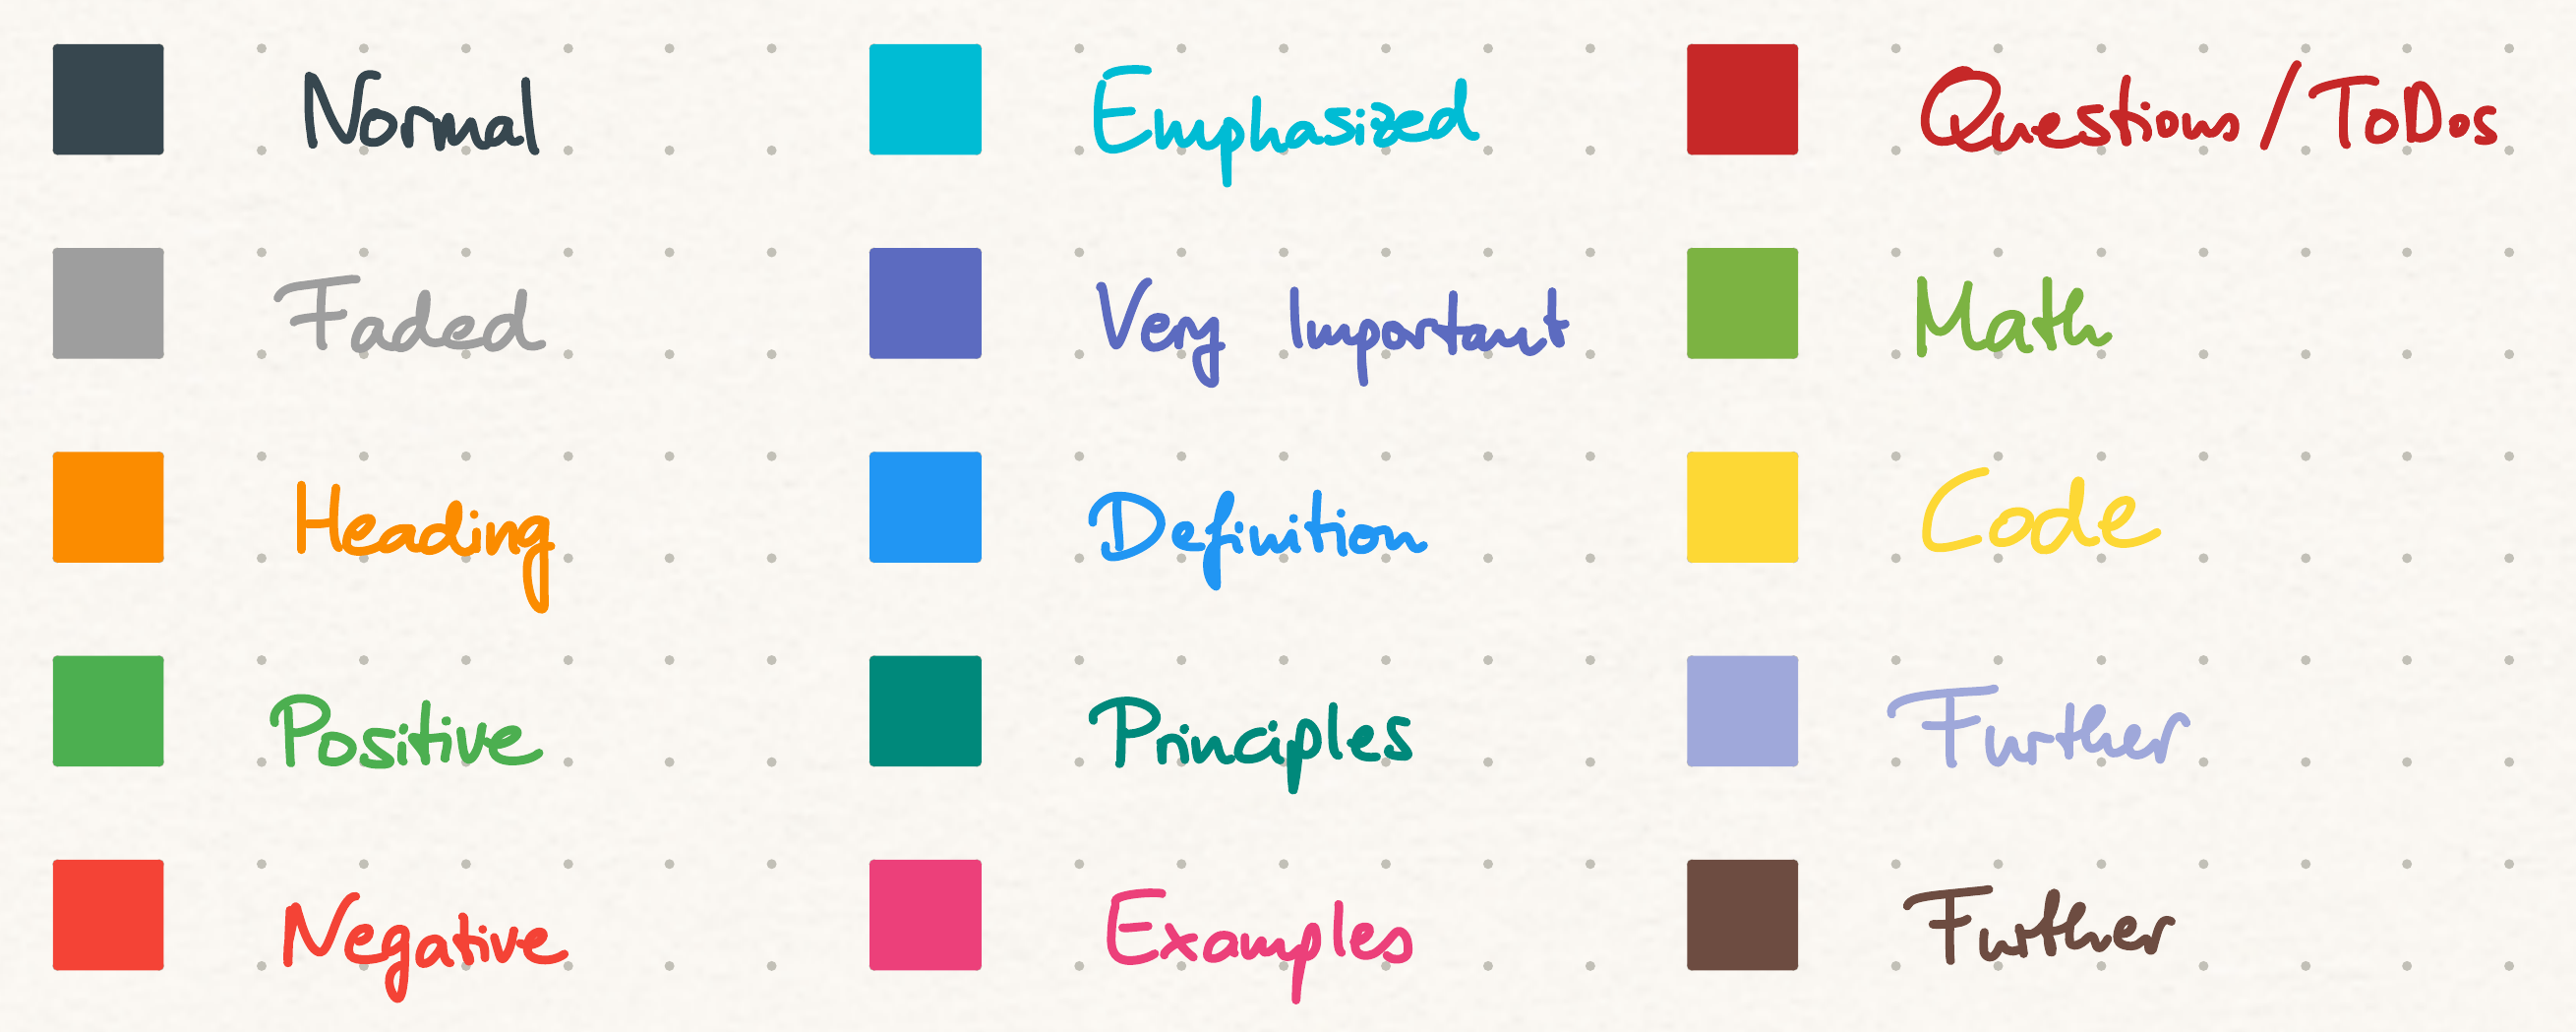
\includegraphics[width=.6\paperwidth]{12_resources/color_scheme.png}
        \caption{The colour scheme I use for highlighting and notetaking.}
    \end{figure}
\end{frame}

\section{Notetaking}
\begin{frame}{Notetaking}
    \begin{itemize}
        \item Handwritten $>$ Typed
    \end{itemize}
    \vspace{1em}
    \begin{table}
    \centering
    \begin{tabular}{p{0.4\textwidth} p{0.5\textwidth}}
        \negative{\textbf{Dont's}}
        \begin{itemize}
            \item Verbatim notes $\Rightarrow$ Shallow processing $\rightarrow$ Can harm learning
        \end{itemize}
        &
        \positive{\textbf{Do's}}
        \begin{itemize}
            \item \red{Generative process}: Summarizing, paraphrasing, organizing, outlining
            \item \red{Efficient notes} = Fewer words to express critical ideas
            \begin{itemize}
                \item Less is more! $\widehat =$ Higher compression
            \end{itemize}
            \item \red{Review} notes, probably more important than creating them
        \end{itemize}
    \end{tabular}
    \end{table}
\end{frame}

\section{Outlining}
\begin{frame}{Outlining}
    \begin{itemize}
        \item Hierarchical representation of main points
        \item \positive{Identify, relate, organize main points}
    \end{itemize}
    \vspace{1em}
    \positive{\textbf{Do's}}
    \begin{itemize}
        \item Outline given by lecturer beforehand benefits learning \grey{($\rightarrow$ Responsibility of lecturer)}
        \begin{itemize}
            \item[$\rightarrow$] Try to comprehend it
        \end{itemize}
        \item Use outline as cue for retrieval practice
        \item Outlining training
    \end{itemize}
\end{frame}

\section{Flash cards}
\begin{frame}{Flash cards}
    \begin{itemize}
        \item \positive{Retain specific, detailed information}
        \item \negative{Difficult to target higher order information}
    \end{itemize}
    \vspace{1em}
    \begin{table}
    \centering
    \begin{tabular}{p{0.4\textwidth} p{0.5\textwidth}}
        \negative{\textbf{Dont's}}
        \begin{itemize}
            \item Just reading the contents
        \end{itemize}
        &
        \positive{\textbf{Do's}}
        \begin{itemize}
            \item Continue practising after getting it correct one time
            \item Spacing
        \end{itemize}
    \end{tabular}
    \end{table}
\end{frame}

\section{Discussion}
\begin{frame}{Discussion}
    \begin{itemize}
        \item Effective ways to augment study strategies: Retrieval, Spacing, instructor assistance
        \begin{itemize}
            \item[$\rightarrow$] \red{Learning strategies are not and either-or decision, but a \emph{spectrum}}
        \end{itemize}
        \item ``New behaviors are attained most efficiently when they are incorporated into preexisting behaviours''
        \begin{itemize}
            \item Implementing completely new methods requires effort
        \end{itemize}
    \end{itemize}
\end{frame}

\section{Now You!}
\begin{frame}{Now You!}
    \begin{itemize}
        \item \emph{Which of your study strategies do you want to make more effective? How?}
    \end{itemize}
\end{frame}

\chapteroverview{12}

\thankyou{Happy Learning!}{sven.ligensa@uni-muenster.de}

\sources

\end{document}
